% appendix

\chapter{追加内容}

\section{三角复习}

\subsection{弧度制}

\begin{itemize}
    \item 定义:
    \begin{equation*}
        \textrm{弧度}=\frac{\textrm{弧长}}{\textrm{半径}}
    \end{equation*}
    \item 特殊值:
    \begin{center}
        \renewcommand\arraystretch{1.2}
        \begin{tabular}{c|c|c|c}
            \hline
            角度         & 弧度        & 角度         & 弧度 \\\hline
            $30^\circ$  & $\frac\pi6$ & $120^\circ$  & $\frac{2\pi}3$\\
            $45^\circ$  & $\frac\pi4$ & $135^\circ$  & $\frac{3\pi}4$\\
            $60^\circ$  & $\frac\pi3$ & $150^\circ$  & $\frac{5\pi}6$\\
            $90^\circ$  & $\frac\pi2$ & $180^\circ$  & $\pi$\\
            \hline
        \end{tabular}
    \end{center}
\end{itemize}

\subsection{三角函数}

\begin{itemize}
    \item 正弦:$\frac{对边}{斜边}$
    \item 余弦:$\frac{邻边}{斜边}$
    \item 正切:$\frac{对边}{邻边}$
    \item 特殊值:
    \begin{center}
        \renewcommand\arraystretch{1.2}
        \begin{tabular}{c|ccc}
            \hline
            角度 & 正弦 & 余弦 & 正切 \\\hline
            $0^\circ$   & $0$              & $1$              & $0$              \\
            $30^\circ$  & $\frac12$        & $\frac{\sqrt3}2$ & $\frac1{\sqrt3}$ \\
            $45^\circ$  & $\frac{\sqrt2}2$ & $\frac{\sqrt2}2$ & $1$              \\
            $60^\circ$  & $\frac{\sqrt3}2$ & $\frac12$        & $\sqrt3$         \\
            $90^\circ$  & $1$              & $0$              & $\infty$         \\
            $180^\circ$ & $0$              & $-1$             & $\infty$         \\
            $\frac\pi2-\theta$ & $\cos\theta$ & $\sin\theta$ & $\frac1{\tan\theta}$\\
            \hline
        \end{tabular}
    \end{center}
\end{itemize}

\section{微分公式}

\subsection{基本初等函数的导数}

\begin{itemize}
    \item 常函数:$y^\prime=0$
    \item 幂函数:$y^\prime=a\cdot x^{a-1}$
    \item 指数函数:$y^\prime=a^x\cdot\ln a$
    \item 对数函数:$\frac1{x\ln a}$
    \item 正弦函数:$(\sin x)^\prime=\cos x$
    \item 余弦函数:$(\cos x)^\prime=-\sin x$
    \item 正切函数:$(\tan x)^\prime=\frac1{\cos^2x}$
\end{itemize}

\subsection{组合函数的导数}

\begin{itemize}
    \item $(f(x)\pm g(x))^\prime=f^\prime(x)\pm g^\prime(x)$
    \item $(f(x)\cdot g(x))^\prime=f^\prime(x)\cdot g(x)+f(x)\cdot g^\prime(x)$
    \item $(\frac{f(x)}{g(x)})^\prime=\frac{f^\prime(x)\cdot g(x)-f(x)\cdot g^\prime(x)}{g^2(x)}$
    \item $f(g(x))^\prime=\frac{df(x)}{dg(x)}\cdot\frac{dg(x)}{dx}=f^\prime(g(x))g^\prime(x)$
\end{itemize}

\section{积分公式}

\begin{itemize}
    \item 常函数:$\int kdx=kx+C$
    \item 幂函数($a\neq-1$):$\int x^adx=\frac{x^{a+1}}{a+1}+C$
    \item 幂函数($a=-1$):$\int x^{-1}dx=\ln|x|+C$
    \item 指数函数:$\int a^xdx=\frac{a^x}{\ln a}+C$
    \item 正弦函数:$\int\sin xdx=-\cos x+C$
    \item 余弦函数:$\int\cos xdx=\sin x+C$
\end{itemize}

\section{力学延伸}

\subsection{平抛运动抛物线验证}

\begin{equation*}
    \begin{cases}
        x=v_0t\\
        y=\frac12gt^2
    \end{cases}\implies
    y=\frac{g}{2{v_0}^2}x^2
\end{equation*}

\subsection{动能推导}

\begin{equation*}
    E_k=\int\vec{F}\cdot d\vec{s}
        =\int m\vec{a}\cdot d\vec{s}
        =\int m\vec{v}\cdot d\vec{v}
        =\frac12mv^2
\end{equation*}

\subsection{机械能守恒推导}

\begin{align*}
    \int_{t_1}^{t_2}mv\frac{dv}{dt}dt&=\int_{t_1}^{t_2}F\frac{dx}{dt}dt\\
    m\int_{v_1}^{v_2}vdv&=\int_{x_1}^{x_2}Fdx\\
    m\int_{v_1}^{v_2}vdv&=\int_{x_0}^{x_2}Fdx-\int_{x_0}^{x_1}Fdx\\
    \Delta E_k&=-\Delta U\\
    \Delta E_k+\Delta U&=0
\end{align*}

\subsection{重力势能推导}

\begin{equation*}
    E_p=W=\int_{-h}^0mg\cdot dx=mgh
\end{equation*}

\subsection{弹力势能推导}

\begin{equation*}
    E_p=W=\int_{x}^0-k\Delta x\cdot d\Delta x=\frac12kx^2
\end{equation*}

\subsection{动量与冲量关系推导}

\begin{equation*}
    \int_{t_1}^{t_2}Fdt
    =\int_{t_1}^{t_2}m\frac{dv}{dt}dt
    =\int_{v_1}^{v_2}mdv
    =mv_2-mv_1
\end{equation*}

\subsection{圆周运动向心加速度推导}

\begin{gather*}
    v=\left(\frac{dx}{dt},\frac{dy}{dt}\right)
    =(-r\omega\sin\omega t,r\omega\cos\omega t)\\
    a=\left(\frac{dv_x}{dt},\frac{dv_y}{dt}\right)
    =(-r\omega^2\cos\omega t,-r\omega^2\sin\omega t)
    =-\omega^2\vec{r}
\end{gather*}

\subsection{单摆周期推导}

\begin{equation*}
    F\approx -mg\sin\theta=-mg\cdot\frac{x}{l}=-\frac{mg}{l}x
\end{equation*}

\subsection{万有引力势能推导}

\begin{equation*}
    E_p=W=\int_r^\infty-G\frac{Mm}{x^2}dx=-G\frac{Mm}{r}
\end{equation*}

\section{热学延伸}

\subsection{理想气体内能公式推导}

如图,气体分子在边长为l的立方体容器内运动、三个方向上的速度均为$v$,假设其与容器壁做弹性碰撞,计算气体压强与分子运动速度的关系。
\begin{figure}[ht!]
    \centering
    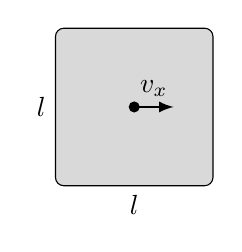
\begin{tikzpicture}
        \filldraw[color=black, fill=gray!30, rounded corners=3pt] (0, 0) rectangle (2, 2);
        \node[below] at (1, 0) {$l$};
        \node[left] at (0, 1) {$l$};
        \draw[thick, -latex] (1, 1) -- node[above] {$v_x$} ++ (0.5, 0) ;
        \fill (1, 1) circle (2pt);
    \end{tikzpicture}
    \caption{气体分子运动与压强}
\end{figure}
由于气体分子在x方向上每折返一次就会与容器壁发生一次碰撞,所以$\Delta t$时间内会与容器壁碰撞$\frac{v\Delta t}{2l}$次。因此这段时间内容器壁受到来自气体分子的冲量为
\begin{equation*}
    2mv\cdot\frac{v_x\Delta t}{2l}=\frac{m{v_x}^2}{l}\Delta t
\end{equation*}
即相当于单个气体分子给予容器壁$F=\frac{m{v_x}^2}{l}$大小的力,相对应的就会有
\begin{equation*}
    P=\frac{F}{l^2}=\frac{m{v_x}^2}{l^3}=\frac{m{v_x}^2}{V}
\end{equation*}
大小的压强。此外,该气体分子也会在y和z方向上做同样的运动,所以其速度的平均值为$\overline{v^2}=\overline{{v_x}^2}+\overline{{v_y}^2}+\overline{{v_z}^2}$。同时,容器内倘若有N个这样的气体分子,那么其压强的总和为
\begin{equation*}
    P=N\cdot\frac{m{v_x}^2}{V}=\frac{Nm\overline{v^2}}{3V}
\end{equation*}
将上述压强值代入理想气体状态方程就可以得到1摩尔该气体分子平均速度的平方。
\begin{gather*}
    PV=nRT\\
    \frac{Nm\overline{v^2}}{3V}V=\frac{N}{N_A}RT\\
    \overline{v^2}=\frac{3RT}{M}
\end{gather*}
那么n摩尔该气体分子的总动能可求。
\begin{equation*}
    n\cdot\frac12M\overline{v^2}=\frac32nRT
\end{equation*}

\subsection{等温变化做功}

\begin{equation*}
    Q_\textrm{吸}=W_\textrm{した}=\int_{V_1}^{V_2}PdV=nRT\cdot\log\frac{V_2}{V_1}
\end{equation*}

\subsection{断热变化PV等式推导}

基于断热变化的热力学第一定律可得
\begin{gather*}
    \Delta U=-W_\textrm{した}\\
    nC_v\Delta T=-PdV
\end{gather*}
简做整理后对两侧分别关于T和V积分
\begin{gather*}
    \int\frac{dT}{T}=-\frac{R}{C_v}\int\frac{dV}{V}\\
    \log T=-\frac{R}{C_v}\log V+c^\prime\\
    T=V^{-\frac{R}{C_v}}\cdot c\\
    TV^{\frac{R}{C_v}}=c
\end{gather*}
在此定义$\gamma=\frac{C_p}{C_v}$,结合$C_p-C_v=R$即有
\begin{equation*}
    TV^{\gamma-1}=c
\end{equation*}
再结合理想气体状态方程就可以得到$PV^\gamma=const$的结论。

\section{波动延伸}

\subsection{波的解析式推导法二}

假设$t=0$时刻的波形为
\begin{equation*}
    y_0=A\sin\left(\frac{2\pi}{\lambda}x\right)
\end{equation*}
那么$t$时间后改图像会向右平移$vt$单位长度,即
\begin{equation*}
    y=A\sin\left(\frac{2\pi}{\lambda}\left(x-vt\right)\right)
    =A\sin\left(2\pi\left(\frac{x}{\lambda}-\frac{t}{T}\right)\right)
\end{equation*}

\subsection{差频公式推导}

设两束声波分别为$y_1=\sin((\omega+\theta)t)$和$y_2=\sin((\omega-\theta)t)$,其中$\omega$远大于$\theta$。那么,根据波的叠加原理可知合成波为
\begin{align*}
    y=&\sin((\omega+\theta)t)+\sin((\omega-\theta)t)\\
    =&(\sin\omega t\cos\theta t+\cos\omega t\sin\theta t)+(\sin\omega t\cos\theta t-\cos\omega t\sin\theta t)\\
    =&(2\cos\theta t)\sin\omega t
\end{align*}
此外,声音的强度与振幅的平方相关,所以合成波的波峰与波谷都会被人耳当成差频接收。因此差频的频率为合成波括号中控制振幅部分频率的两倍。
\begin{align*}
    f=&2\times\frac{\theta}{2\pi}\\
    =&\frac{\omega_1-\omega_2}{2\pi}\\
    =&f_1-f_2
\end{align*}

\subsection{光程公式推导}

使波长为$\lambda$的波在折射率为$n$的介质中传播$l$长的距离,那么在这段空间中存在$\frac{l}{\lambda^\prime}=\frac{nl}{\lambda}$个波。倘若把这些波换算到真空中($n=1$)中,则需要
\begin{equation*}
    L=\frac{l}{\lambda^\prime}\times\lambda=nl
\end{equation*}
的距离。称$L$为光程,满足$L=nl$。

\subsection{双缝干涉光程差推导}

\begin{equation*}
    |S_1P-S_2P|=S_2H\approx d\sin\theta\approx d\tan\theta=\frac{dx}{l}
\end{equation*}

\subsection{薄膜干涉光程差推导}

根据三角关系以及折射定律可知
\begin{equation*}
    \begin{cases}
        AH=AB\sin\phi\\
        BD=AB\sin\theta\\
        \sin\theta=n\sin\phi
    \end{cases}
\end{equation*}
即$n\cdot AH=BD$,$AH$与$BD$等光程。也就是说两束光到B点前的光程差为$HC+BC$。在此,将$BC$向下对称翻转得到$BC^\prime$,因而
\begin{equation*}
    HC+BC=HC+BC^\prime=HC^\prime=2d\cos\phi
\end{equation*}
由于这个距离是折射率为$n$的介质中的,所以其真空中等效的光程为$2nd\cos\phi$。

\subsection{牛顿环干涉光程差推导}

结合勾股定理关于$R$、$r$、$d$列方程即可。
\begin{align*}
    R^2=&r^2+(R-d)^2\\
    r^2=&(2R-d)d\\
    \downarrow&\quad R\gg d\\
    r^2=&2Rd
\end{align*}

\section{电磁延伸}

\subsection{点电荷电势推导}

\begin{gather*}
    U=\int_r^\infty k\frac{Qq}{x^2}dx=k\frac{Qq}{r}\\
    V=\frac{U}{q}=k\frac{Q}{r}
\end{gather*}

\subsection{电容器储能公式推导}

\begin{equation*}
    U=\int_0^Q\frac{q}{C}dq=\frac{Q^2}{2C}
\end{equation*}

\subsection{电容器储能损耗推导}

假设电路中除电容器以外的外阻为$R$,则回路方程为
\begin{equation*}
    E=RI+\frac{Q}{C}\implies
    \frac{dQ}{dt}=I=\frac{E-\frac{Q}{C}}{R}
\end{equation*}
对等式两边积分可得电荷量随时间变化的函数
\begin{gather*}
    \int\frac{dQ}{E-\frac{Q}{C}}=\int\frac{dt}{R}\\
    -C\log\left\lvert E-\frac{Q}{C}\right\rvert=\frac{t}{R}+\gamma\\
    E-\frac{Q}{C}=\Gamma\exp\left(\frac{t}{RC}\right)\quad\left(\Gamma=\exp\left(-\frac{\gamma}{C}\right)\right)\\
\end{gather*}
根据初始条件$(t,Q)=(0,0)$可得$\Gamma=E$,因此
\begin{equation*}
    Q(t)=CE\left(1-\exp\left(-\frac{t}{RC}\right)\right)
\end{equation*}
最后使用$W=I^2Rt$积分求解即可
\begin{gather*}
    I=\frac{dQ}{dt}=\frac{E}{R}\exp\left(-\frac{t}{RC}\right)\\
    W=\int_0^\infty I^2Rdt=\frac12CE^2
\end{gather*}

\subsection{直线电流磁场推导}

根据Biot-Savart定律可得
\begin{align*}
    \mathbf{B}=&\frac{\mu_0}{4\pi}\int_{-\infty}^{\infty}\mathbf{J}\times\frac{\mathbf{r}-\mathbf{l}}{|\mathbf{r}-\mathbf{l}|^3}d^3l\\
    =&\frac{\mu_0I}{4\pi}\int_{-\infty}^{\infty}d\mathbf{l}\times\frac{\mathbf{r}-\mathbf{l}}{|\mathbf{r}-\mathbf{l}|^3}
\end{align*}
设$(0,0,r_z)$为矢量基准点,则可简记$r=(r_x,r_y,0)$
\begin{align*}
    \mathbf{B}=&\frac{\mu_0I}{4\pi}\int_{-\infty}^{\infty}dl\cdot e_z\times\frac{r_xe_x+r_ye_y-le_z}{|r^2+l^2|^{3/2}}\\
    =&\frac{\mu_0I}{4\pi}\int_{-\infty}^{\infty}dl\frac{r_xe_y-r_ye_x}{|r^2+l^2|^{3/2}}
\end{align*}
关于$l$求解反常积分可得
\begin{align*}
    \mathbf{B}=&\frac{\mu_0I}{4\pi}\left[\frac{l(r_xe_y-r_ye_x)}{r^2\sqrt{r^2+l^2}}\right]_{-\infty}^{\infty}\\
    =&\frac{\mu_0I}{2\pi r^2}(r_xe_y-r_ye_x)
\end{align*}
将结果改写为位置向量的形式
\begin{equation*}
    \mathbf{B}=\frac{\mu_0I}{2\pi r^2}(-r_y,r_x,0)
\end{equation*}
即大小为$B=\frac{\mu_0I}{2\pi r}$,方向与$\mathbf{r}$垂直的磁场

\subsection{环形电流磁场推导}

设位于xy平面上的环形电流半径为$r$,计算z轴上点$\mathbf{z}=(0,0,z)$处的磁场。则根据Biot-Savart定律$\mathbf{l}=(l\cos\phi,l\sin\phi,0)$处的微小电流产生的磁场即为
\begin{align*}
    d\mathbf{B}=&\frac{\mu_0I}{4\pi}\frac{d\mathbf{l}\times(\mathbf{z}-\mathbf{l})}{|\mathbf{z}-\mathbf{l}|^3}\\
    =&\frac{\mu_0I}{4\pi|\mathbf{z}-\mathbf{l}|^3}(-\sin\phi,\cos\phi,0)dl\times(-l\cos\phi,-l\sin\phi,r)\\
    =&\frac{\mu_0I}{4\pi|\mathbf{z}-\mathbf{l}|^3}(r\cos\phi,r\sin\phi,l)dl
\end{align*}
分别关于xyz三个方向积分可得
\begin{align*}
    \begin{cases}
        B_x=\frac{\mu_0}{4\pi}\oint\frac{z\cos\phi}{|\mathbf{z}-\mathbf{l}|^3}dl
        =\frac{\mu_0}{4\pi}\int_0^{2\pi}\frac{z\cos\phi}{|\mathbf{z}-\mathbf{l}|^3}ld\phi=0\\
        B_y=\frac{\mu_0}{4\pi}\oint\frac{z\sin\phi}{|\mathbf{z}-\mathbf{l}|^3}dl=0\\
        B_z=\frac{\mu_0}{4\pi}\oint\frac{l}{|\mathbf{z}-\mathbf{l}|^3}dl
        =\frac{\mu_0}{4\pi}\oint\frac{ldl}{(z^2+l^2)^{3/2}}=\frac{\mu_0Il^2}{2(z^2+l^2)^{3/2}}\\
    \end{cases}
\end{align*}
可见除$B_z$以外的磁场均为0,并且当$z=0$时$B_z=\frac{\mu_0I}{2l}$的确成立

\chapter{历年考点}

\section{年份题号对照表}

\begin{changemargin}{-2.5cm}{-2.5cm}
    \begin{center}
        \small
        \renewcommand\arraystretch{1.2}
        \begin{tabular}{c*{19}{|c}}
            \hline
            章节&\multicolumn{6}{|c}{力学}&\multicolumn{3}{|c}{热学}&\multicolumn{3}{|c}{波动}&\multicolumn{6}{|c}{电磁}&\multicolumn{1}{|c}{原子}\\\hline
            题号&1&2&3&4&5&6&7&8&9&10&11&12&13&14&15&16&17&18&19\\\hline
            21A&1.2&2.2&1.2&2.2&3.2&3.1&
                1&2.2&2.3&
                1.1&2.3&3.1&
                1.1&1.3&2.1&3.1&3.2&4.1&
                3\\\hline
            20B&1.3&1.2&2.2&2&3.1&3.3&
                1&2.1&2.3&
                1.1&2.3&3.1&
                1.1&1.2&1.3&2.3&3.3&4.1&
                2\\\hline
            19A&1.3&1.2&1.2&2&3.2&3.3&
                1&2.1&2.2&
                1.1&2.3&3.1&
                1.1&1.1&2.1&1.3&3.1&3.3&
                -\\\hline
            18B&1.2&1.1&2.1&2.2&3.1&3.2&
                1&2.1&2.2&
                1.1&2.2&3.2&
                1&1.3&2.3&3.2&3.3&4.1&
                2\\\hline
            18A&1.2&1.2&2.2&2.2&2.1&3.2&
                1&2.1&-&
                1.1&2.2&3.1&
                1.1&1.3&2.3&3.1&3.2&4.1&
                2\\\hline
            17B&1.2&1.2&2.1&2&2.1&3.2&
                1&2.1&2.3&
                1.1&2.2&3.2&
                1.1&1.2&1.3&2.1&3.1&3.2&
                3\\\hline
            17A&1.2&1.2&2.2&3.1&2&3.3&
                1&2.1&2.2&
                1.1&2.3&3.1&
                1.1&1.3&2.3&3.1&3.2&4.1&
                3\\\hline
            16B&1.2&1.1&1.2&2&2.2&3.1&
                1&2.2&2.3&
                1.1&2.2&3.1&
                1.1&1.2&1.3&2.3&2.3&3.2&
                3\\\hline
            16A&1.2&1.2&2&2.2&3.2&3.1&
                1&2.1&2.3&
                1.3&2.2&3.2&
                1.1&1.2&2.1&1.3&3.1&3.3&
                2\\\hline
            15B&1.3&1.1&1.2&2.1&2.2&3.1&
                1&2.2&2.2&
                1.3&1.2&3.2&
                1.2&1.3&2.1&3.1&3.2&4.1&
                1\\\hline
            15A&1.3&1.2&2.2&2.1&2.2&3.1&
                1&2.2&2.3&
                1.1&1.2&3.1&
                1.1&1.3&2.3&3.1&3.2&4.1&
                1\\\hline
        \end{tabular}
    \end{center}
\end{changemargin}
以上为2015年至今所有真题的知识点一览表,每个单元格内是对应的小节号。

\section{章节频次对照表}

\begin{center}
    \renewcommand\arraystretch{1.2}
    \begin{minipage}{0.48\textwidth}
        \centering
        \begin{tabular}{c|c|c}
            \hline
            小节&内容&次数\\\hline
            \multicolumn{3}{c}{力学}\\\hline
            1.1.1&速度加速度&3\\\hline
            1.1.2&运动与力&18\\\hline
            1.1.3&刚体与力&4\\\hline
            1.2.1&能量&12\\\hline
            1.2.2&动量&18\\\hline
            1.3.1&圆周运动&8\\\hline
            1.3.2&简谐振动&6\\\hline
            1.3.3&天体运动&3\\\hline
            \multicolumn{3}{c}{热学}\\\hline
            2.1&热与能量&11\\\hline
            2.2.1&气体法则&7\\\hline
            2.2.2&热力学第一定律&8\\\hline
            2.2.3&气体状态变化&6\\\hline
            \multicolumn{3}{c}{波动}\\\hline
            3.1.1&波的传播&9\\\hline
            3.1.2&波的干涉&2\\\hline
            3.1.3&衍射·反射·折射&2\\\hline
            3.2.1&声波&0\\\hline
        \end{tabular}
    \end{minipage}
    \begin{minipage}{0.48\textwidth}
        \centering
        \begin{tabular}{c|c|c}
            \hline
            小节&内容&次数\\\hline
            3.2.2&多普勒效应&5\\\hline
            3.2.3&共振现象&4\\\hline
            3.3.1&光的折射&7\\\hline
            3.3.2&光的干涉&4\\\hline
            \multicolumn{3}{c}{电磁}\\\hline
            4.1.1&电场&11\\\hline
            4.1.2&电势&6\\\hline
            4.1.3&电容器&11\\\hline
            4.2.1&欧姆定律&5\\\hline
            4.2.3&直流电路&7\\\hline
            4.3.1&磁场&8\\\hline
            4.3.2&安培力&7\\\hline
            4.3.3&洛伦兹力&4\\\hline
            4.4.1&电磁感应&7\\\hline
            4.4.2&交流电&0\\\hline
            \multicolumn{3}{c}{原子}\\\hline
            5.1&原子模型&2\\\hline
            5.2&光与电磁波&4\\\hline
            5.3&核反应&4\\\hline
        \end{tabular}
    \end{minipage}
\end{center}

\chapter{配图一览}

\makeatletter
\begin{multicols}{2}
    \@starttoc{lof}
\end{multicols}
\makeatother
